% Auto-generated LaTeX includes for figures and tables
% 问题一
\begin{figure}[H]
\centering
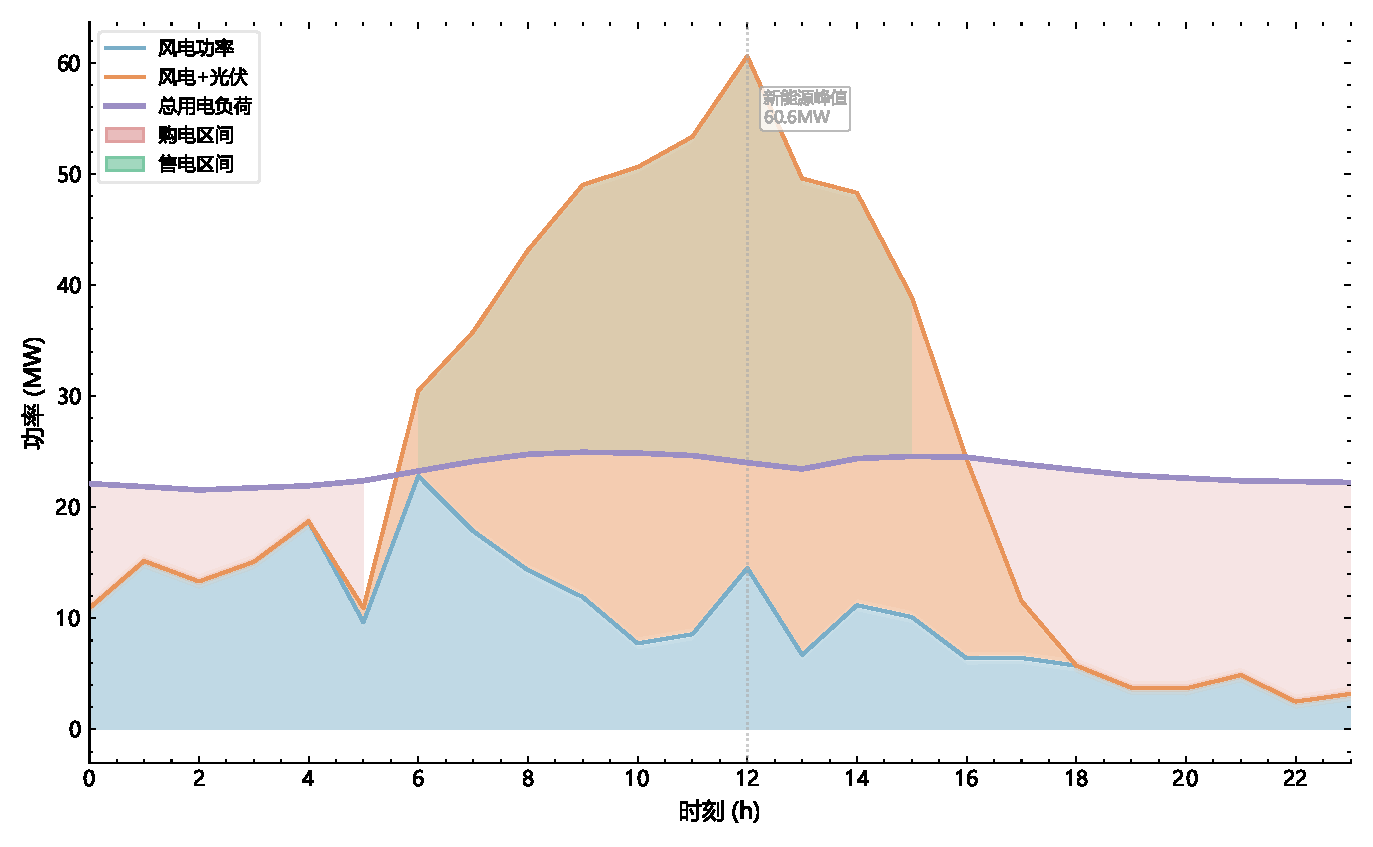
\includegraphics[width=\textwidth]{figures/fig_q1_power_balance.pdf}
\caption{典型日功率平衡曲线（风电、光伏、用电负荷、购售电区间）}
\label{fig:q1_power_balance}
\end{figure}

\begin{figure}[H]
\centering
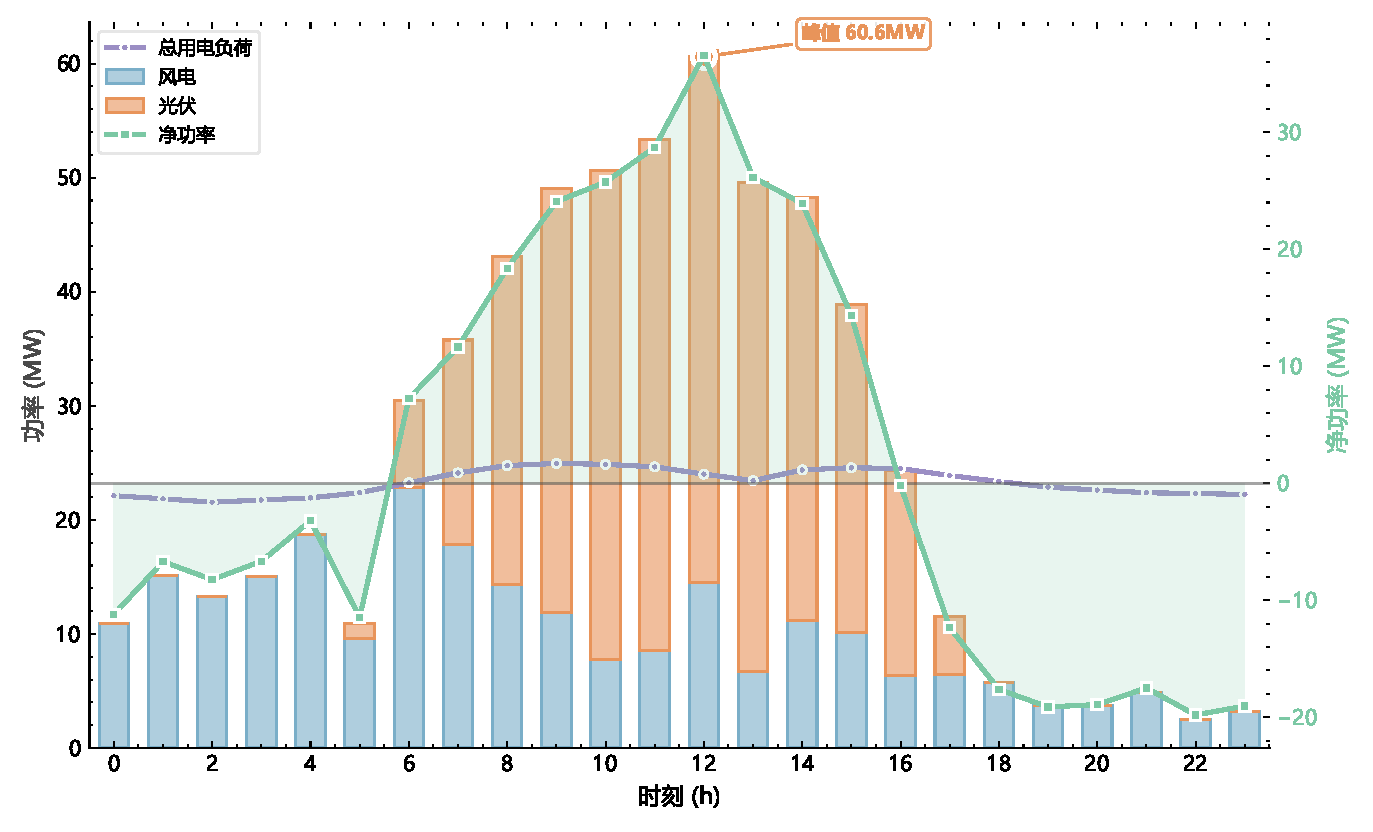
\includegraphics[width=\textwidth]{figures/fig_q1_power_detail.pdf}
\caption{风光发电与负荷功率对比及净功率变化}
\label{fig:q1_power_detail}
\end{figure}

\begin{table}[H]
\centering
\caption{问题一典型日各项电量指标及绿电指标汇总}
\begin{tabular}{lcc}
\toprule
指标 & 数值 & 是否达标 \\
\midrule
总用电量 (MWh) & 558.72 & — \\
新能源发电量 (MWh) & 603.45 & — \\
网购电量 (MWh) & 172.04 & — \\
上网电量 (MWh) & 216.77 & — \\
自发自用电量 (MWh) & 386.68 & — \\
\midrule
自发自用比 R1 (>60\%) & 28.16\% & \textbf{否} \\
绿电比例 R2 (>30\%) & 69.21\% & 是 \\
上网比例 R3 (<20\%) & 35.92\% & \textbf{否} \\
吨氨成本 (元/吨) & 4322.34 & — \\
\bottomrule
\end{tabular}
\end{table}

% 问题二
\begin{figure}[H]
\centering
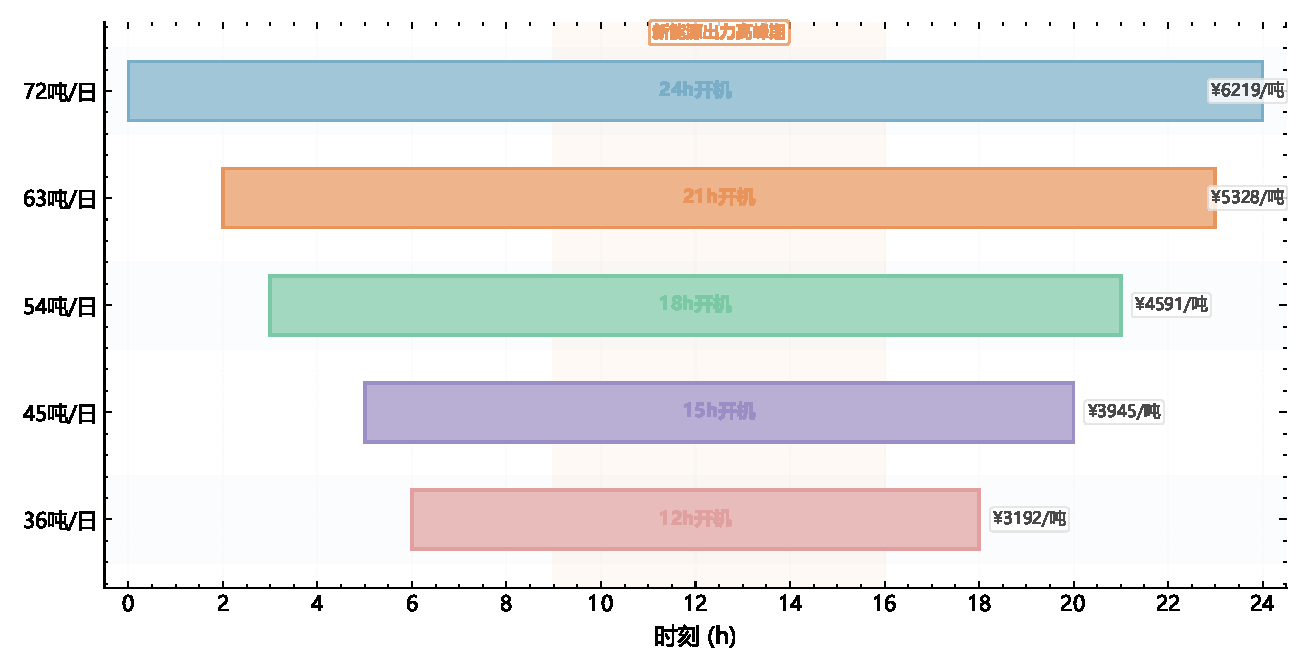
\includegraphics[width=\textwidth]{figures/fig_q2_gantt.pdf}
\caption{各产量水平最优开机时段安排}
\label{fig:q2_gantt}
\end{figure}

\begin{figure}[H]
\centering
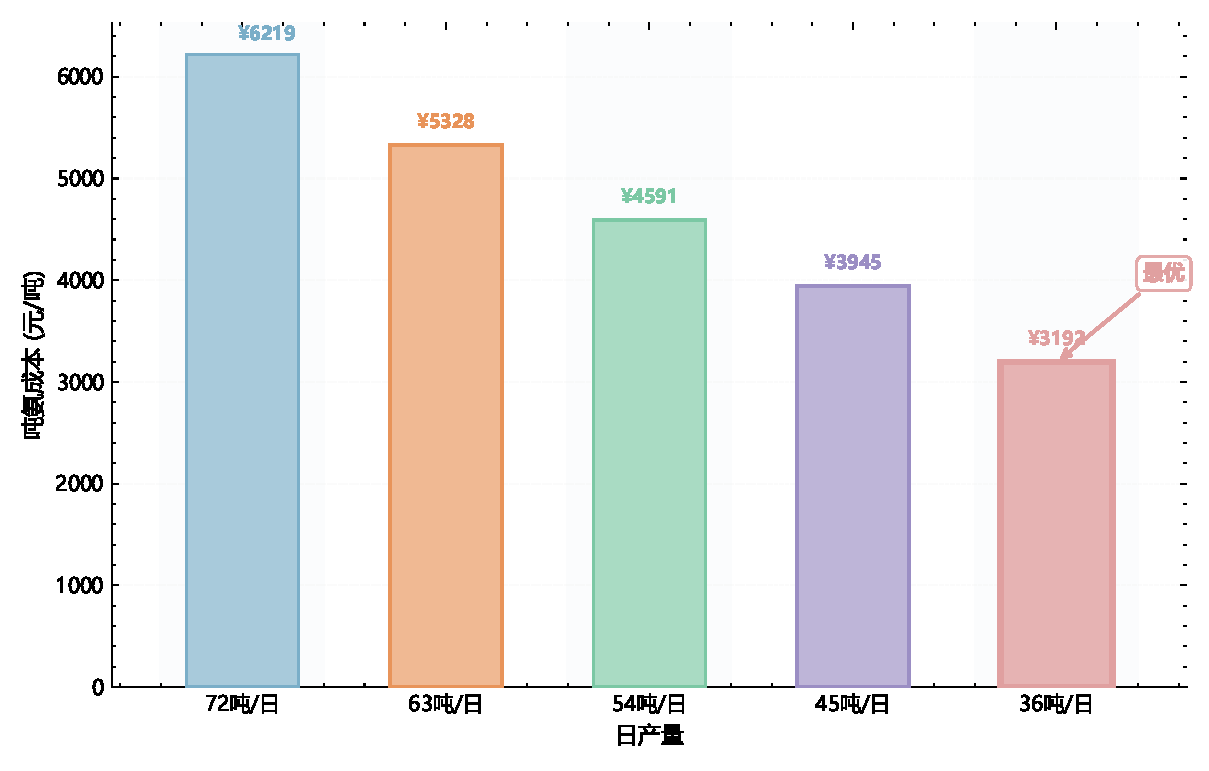
\includegraphics[width=0.85\textwidth]{figures/fig_q2_cost_compare.pdf}
\caption{不同产量水平的吨氨成本对比}
\label{fig:q2_cost_compare}
\end{figure}

\begin{figure}[H]
\centering
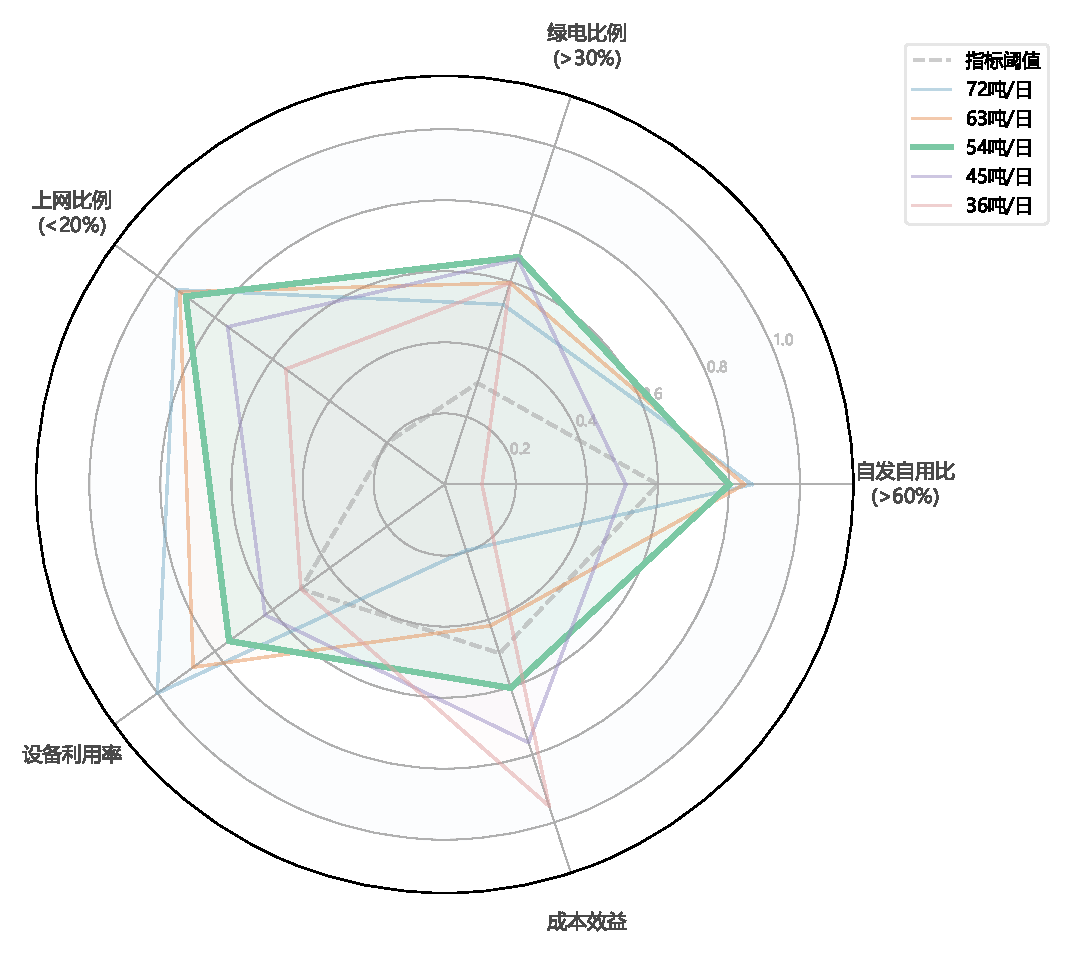
\includegraphics[width=0.75\textwidth]{figures/fig_q2_indicators.pdf}
\caption{各产量水平绿电指标雷达图对比}
\label{fig:q2_indicators}
\end{figure}

\begin{table}[H]
\centering
\caption{典型场景各产量最优方案对比}
\resizebox{\textwidth}{!}{
\begin{tabular}{ccccccc}
\toprule
日产量(吨/日) & 开机时段(h) & 吨氨成本(元/吨) & R1(\%) & R2(\%) & R3(\%) & 达标情况 \\
\midrule
72 & 24 & 6219.14 & 86.52 & 53.26 & 6.74 & 全满足 \\
63 & 21 & 5328.06 & 84.33 & 59.66 & 7.83 & 全满足 \\
54 & 18 & 4591.27 & 80.16 & 67.30 & 9.92 & 全满足 \\
45 & 15 & 3944.54 & 50.98 & 66.67 & 24.51 & 不满足 \\
36 & 12 & 3191.67 & 10.50 & 59.68 & 44.75 & 不满足 \\
\bottomrule
\end{tabular}}
\end{table}

\begin{figure}[H]
\centering
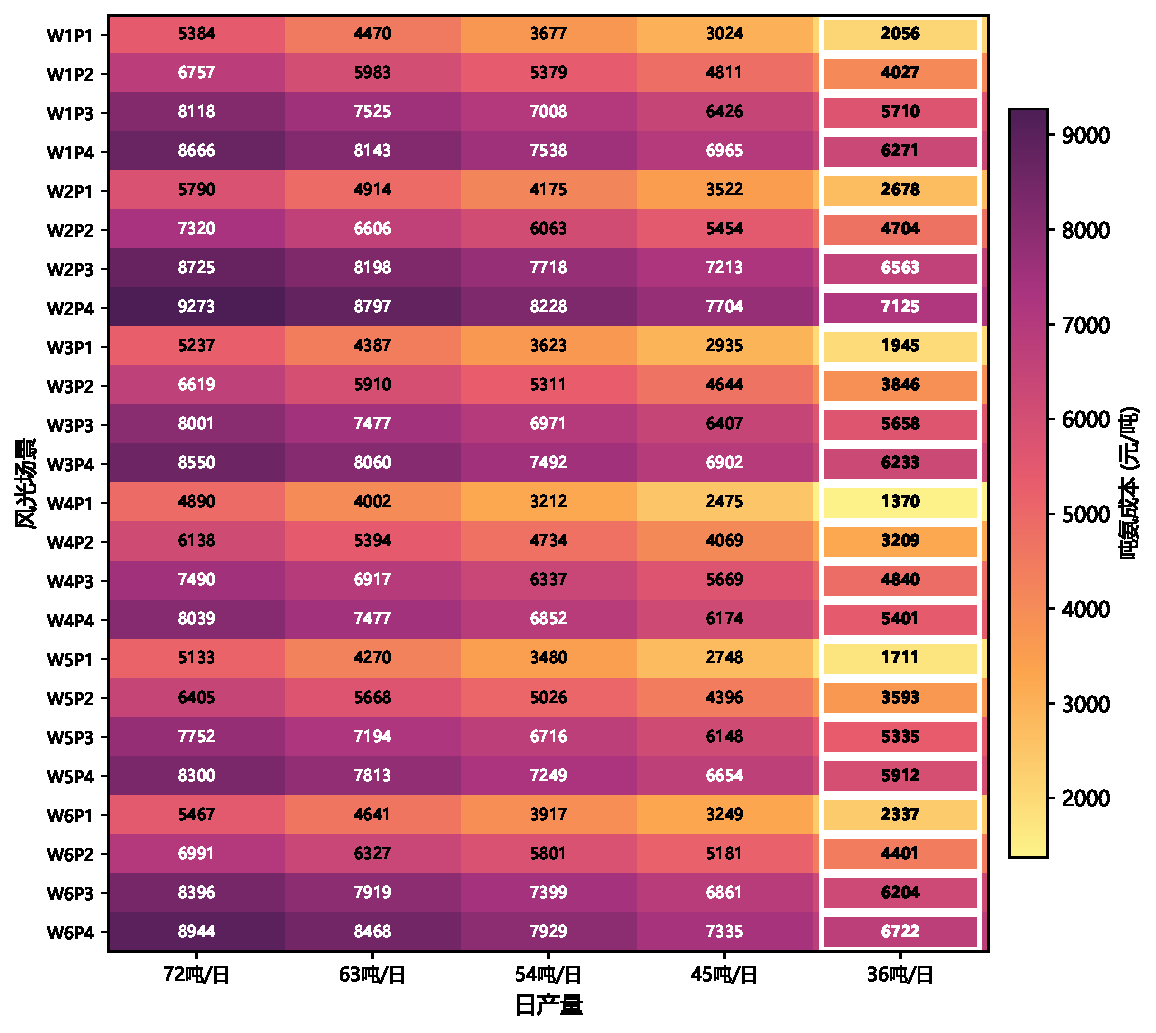
\includegraphics[width=\textwidth]{figures/fig_q2_scenario_heatmap.pdf}
\caption{24场景$\times$5产量的吨氨成本热力图}
\label{fig:q2_scenario_heatmap}
\end{figure}

\begin{figure}[H]
\centering
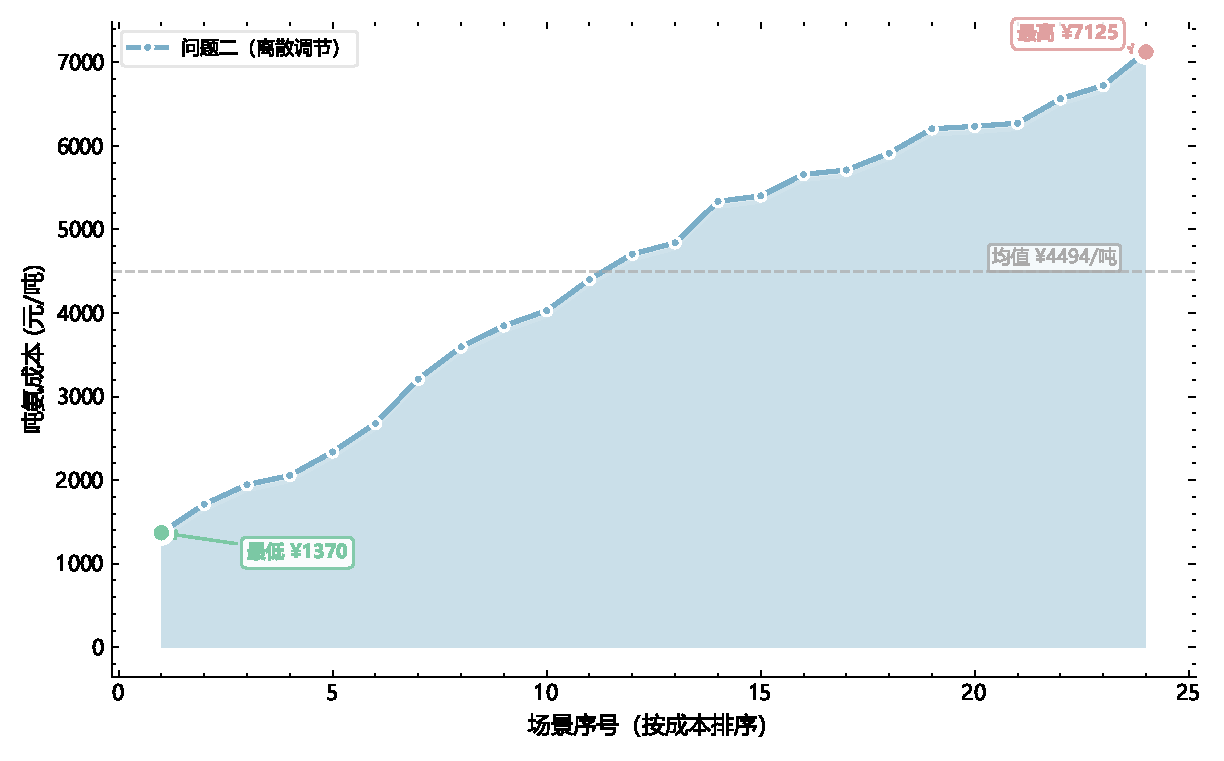
\includegraphics[width=\textwidth]{figures/fig_q2_annual_cost.pdf}
\caption{全年吨氨成本分布曲线（问题二，离散调节）}
\label{fig:q2_annual_cost}
\end{figure}

\begin{table}[H]
\centering
\caption{24场景全年绿电指标统计（问题二）}
\begin{tabular}{lccc}
\toprule
类别 & 场景数 & 占比 & 说明 \\
\midrule
全满足 & 0 & 0.0\% & 三项指标均达标 \\
部分满足 & 21 & 87.5\% & 部分指标达标 \\
全不满足 & 3 & 12.5\% & 三项指标均不达标 \\
\midrule
全年吨氨成本 & \multicolumn{3}{c}{\textyen 4493.82/吨} \\
\bottomrule
\end{tabular}
\end{table}

% 问题三
\begin{figure}[H]
\centering
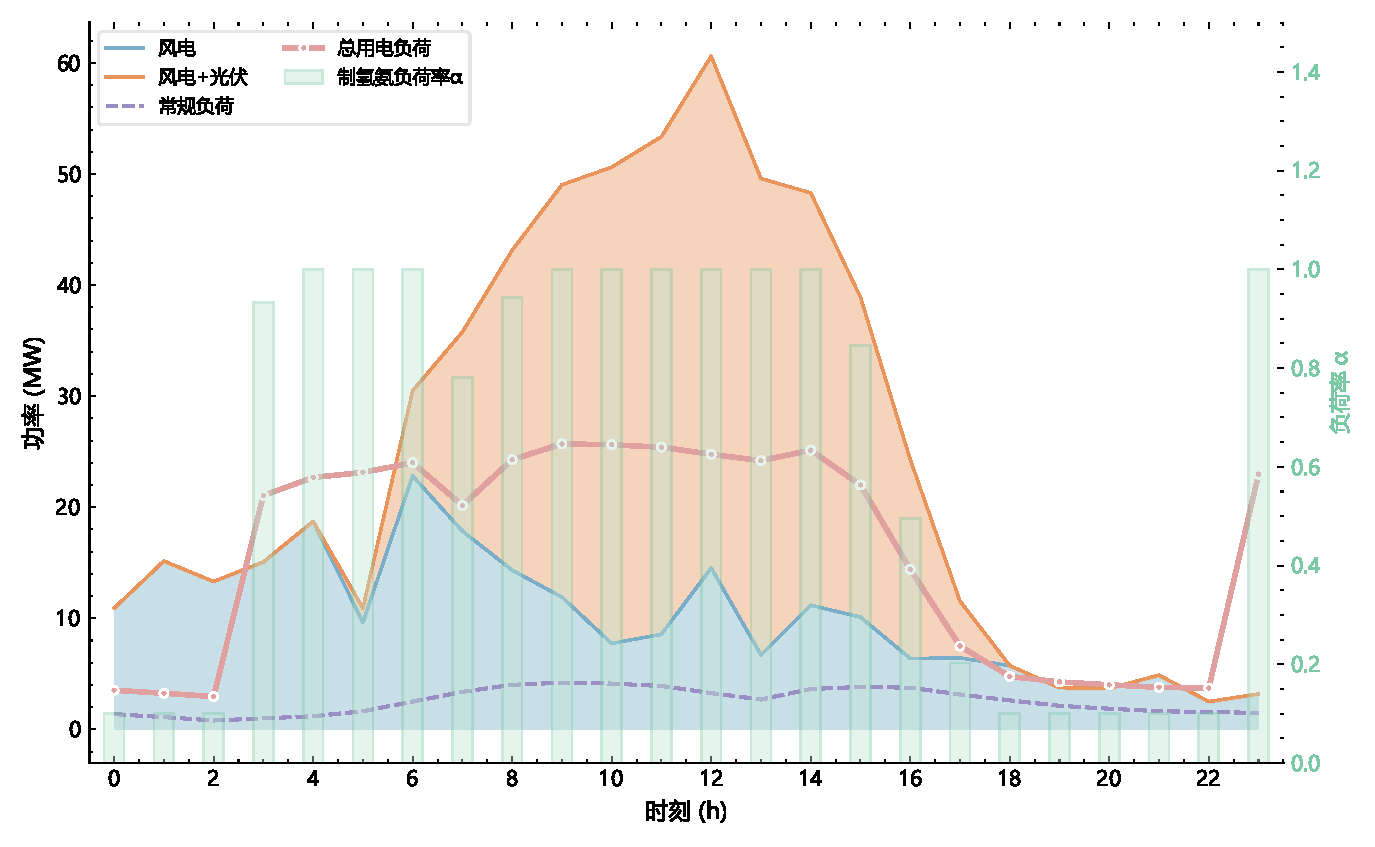
\includegraphics[width=\textwidth]{figures/fig_q3_dispatch.pdf}
\caption{典型场景连续调度功率分配方案}
\label{fig:q3_dispatch}
\end{figure}

\begin{figure}[H]
\centering
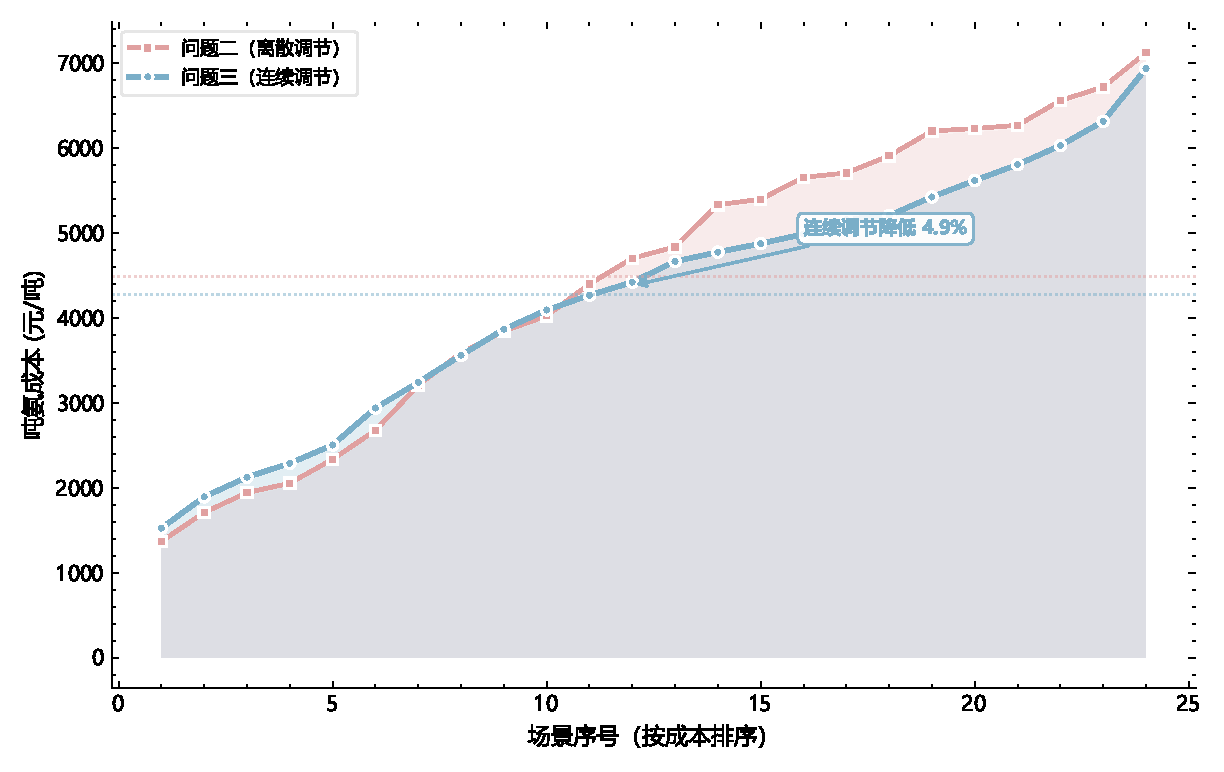
\includegraphics[width=\textwidth]{figures/fig_q3_annual_cost.pdf}
\caption{全年吨氨成本分布曲线（问题二与问题三对比）}
\label{fig:q3_annual_cost}
\end{figure}

\begin{table}[H]
\centering
\caption{问题三24场景连续调节最优方案汇总（部分场景）}
\resizebox{\textwidth}{!}{
\begin{tabular}{ccccccc}
\toprule
场景 & 最优产量(吨/日) & 吨氨成本(元/吨) & R1(\%) & R2(\%) & R3(\%) & 达标情况 \\
\midrule
W1P1 & 36 & 2290 & 32.7 & 90.5 & 33.7 & 部分 \\
W1P2 & 36 & 4096 & 81.9 & 81.9 & 9.0 & 全满足 \\
W1P3 & 36 & 5162 & 98.5 & 59.9 & 0.8 & 全满足 \\
W1P4 & 36 & 5808 & 100.0 & 48.8 & 0.0 & 全满足 \\
W2P1 & 36 & 2941 & 30.9 & 77.2 & 34.6 & 部分 \\
W2P2 & 36 & 4668 & 51.8 & 54.4 & 24.1 & 部分 \\
W2P3 & 36 & 6033 & 100.0 & 42.0 & 0.0 & 全满足 \\
W2P4 & 36 & 6940 & 100.0 & 30.4 & 0.0 & 全满足 \\
W3P1 & 36 & 2127 & 33.2 & 93.1 & 33.4 & 部分 \\
W3P2 & 36 & 3869 & 56.3 & 73.1 & 21.8 & 部分 \\
\bottomrule
\end{tabular}}
\end{table}

\begin{figure}[H]
\centering
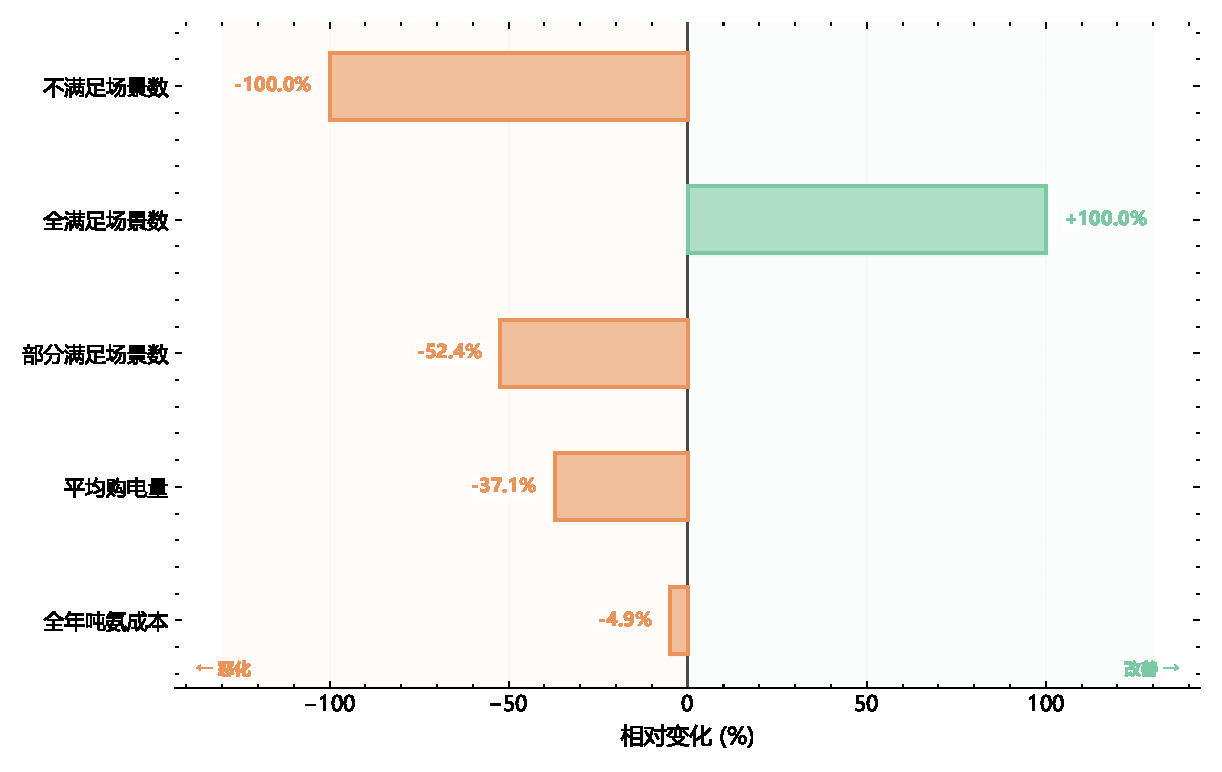
\includegraphics[width=0.9\textwidth]{figures/fig_q3_compare.pdf}
\caption{问题三相对问题二各指标变化量}
\label{fig:q3_compare}
\end{figure}

\begin{table}[H]
\centering
\caption{问题二与问题三关键指标对比}
\begin{tabular}{lccc}
\toprule
指标 & 问题二（离散） & 问题三（连续） & 变化 \\
\midrule
全年吨氨成本 (元/吨) & 4493.82 & 4274.18 & -4.9\% \\
全满足场景数 & 0 & 14 & +14 \\
部分满足场景数 & 21 & 10 & -11 \\
全不满足场景数 & 3 & 0 & -3 \\
\bottomrule
\end{tabular}
\end{table}

% 问题四
\begin{figure}[H]
\centering
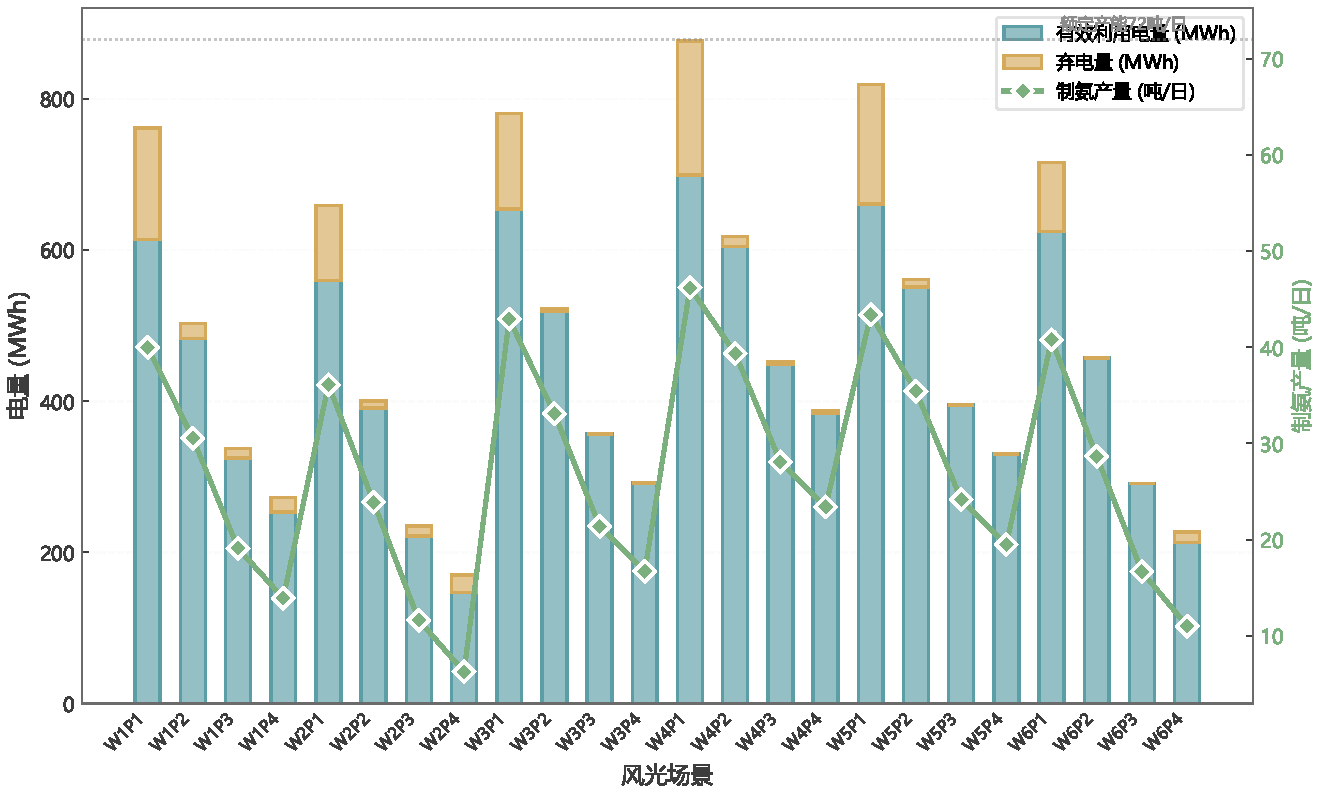
\includegraphics[width=\textwidth]{figures/fig_q4_offgrid_production.pdf}
\caption{24场景离网产量与电量利用分布}
\label{fig:q4_offgrid_production}
\end{figure}

\begin{table}[H]
\centering
\caption{离网各场景产量与成本（部分场景）}
\resizebox{\textwidth}{!}{
\begin{tabular}{cccccc}
\toprule
场景 & 制氨产量(吨/日) & 吨氨成本(元/吨) & 风光利用率(\%) & 弃电量(MWh) & 发电量(MWh) \\
\midrule
W1P1 & 39.98 & 4143 & 80.6 & 147.9 & 761.8 \\
W1P2 & 30.54 & 3893 & 96.0 & 20.1 & 503.2 \\
W1P3 & 19.09 & 4185 & 96.3 & 12.6 & 337.4 \\
W1P4 & 13.91 & 4565 & 92.8 & 19.7 & 272.8 \\
W2P1 & 36.10 & 3982 & 85.0 & 99.0 & 658.9 \\
W2P2 & 23.88 & 3867 & 97.7 & 9.4 & 400.3 \\
W2P3 & 11.62 & 4477 & 94.4 & 13.3 & 234.6 \\
W2P4 & 6.25 & 5649 & 86.6 & 22.9 & 169.9 \\
W3P1 & 42.92 & 4040 & 83.8 & 126.4 & 780.8 \\
W3P2 & 33.10 & 3807 & 99.3 & 3.7 & 522.3 \\
\bottomrule
\end{tabular}}
\end{table}

\begin{figure}[H]
\centering
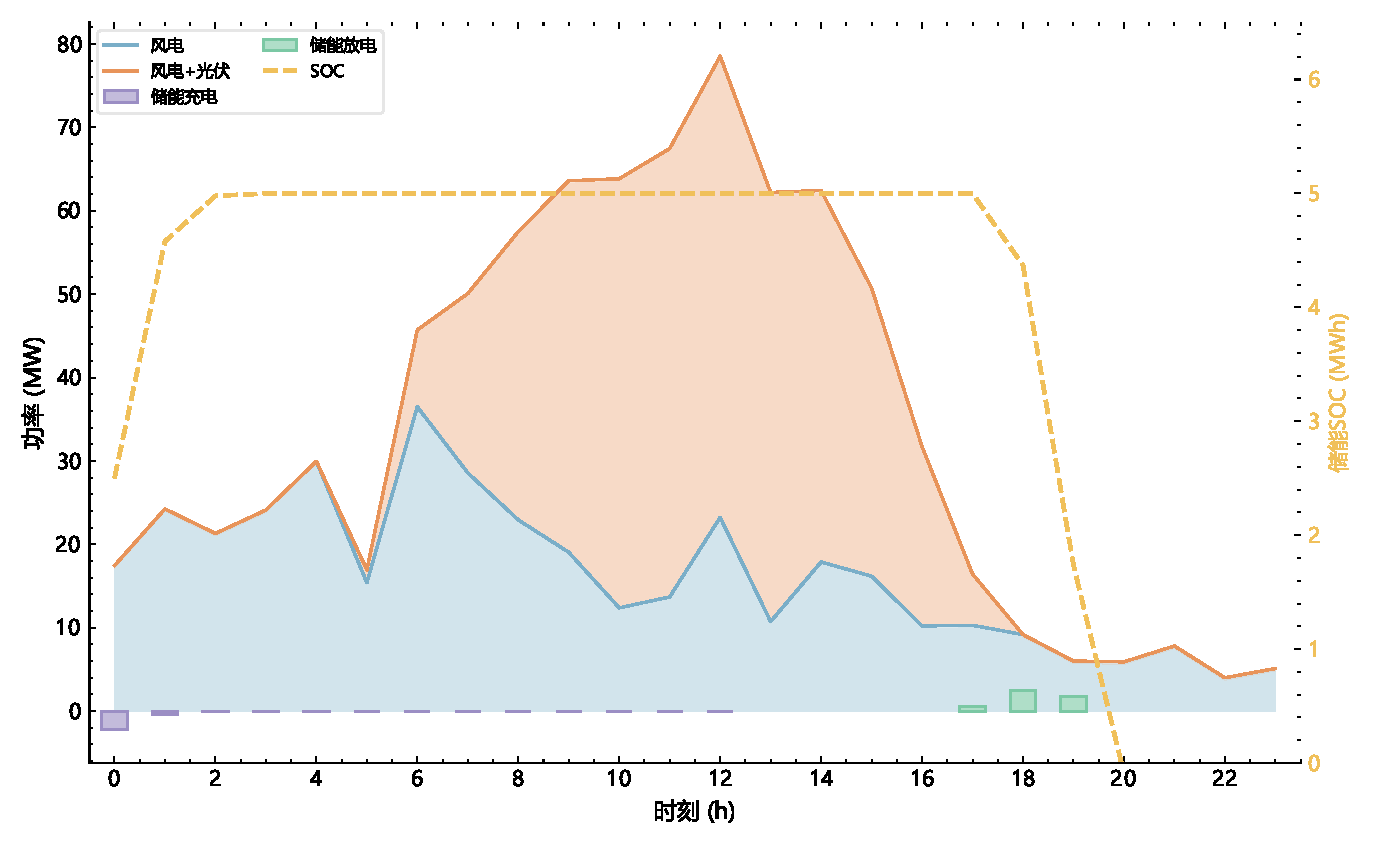
\includegraphics[width=\textwidth]{figures/fig_q4_storage_dispatch.pdf}
\caption{最大弃电场景储能充放电调度方案}
\label{fig:q4_storage_dispatch}
\end{figure}

\begin{table}[H]
\centering
\caption{储能配置方案及效果}
\begin{tabular}{lc}
\toprule
参数 & 数值 \\
\midrule
最优储能容量 (MWh) & 5 \\
目标场景 & W4P1 \\
配储后制氨产量 (吨/日) & 46.51 \\
配储后吨氨成本 (元/吨) & 4189.10 \\
全年制氨总量 (吨) & 9831.0 \\
平均产能利用率 & 37.93\% \\
\bottomrule
\end{tabular}
\end{table}

\begin{figure}[H]
\centering
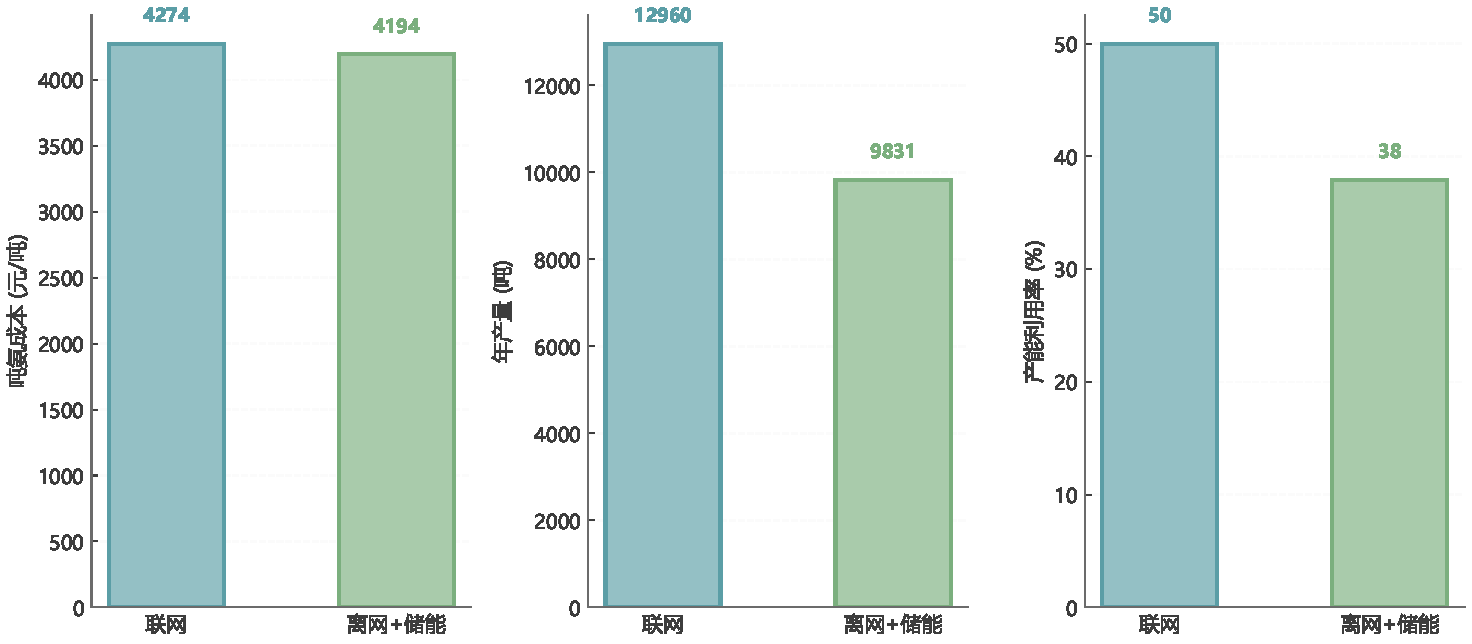
\includegraphics[width=\textwidth]{figures/fig_q4_economics.pdf}
\caption{离网与联网运行模式经济性对比}
\label{fig:q4_economics}
\end{figure}

\begin{table}[H]
\centering
\caption{离网与联网运行模式全年经济性对比}
\begin{tabular}{lccc}
\toprule
指标 & 联网运行 & 离网+储能 & 差异 \\
\midrule
全年吨氨成本 (元/吨) & 4274.18 & 4194.02 & -1.9\% \\
全年制氨总量 (吨) & 12960 & 9831 & -24.1\% \\
产能利用率 (\%) & 50.0 & 37.9 & -12.1 \\
系统支撑成本 (万元) & — & — & 2516 \\
\bottomrule
\end{tabular}
\end{table}

% 灵敏度分析
\begin{figure}[H]
\centering
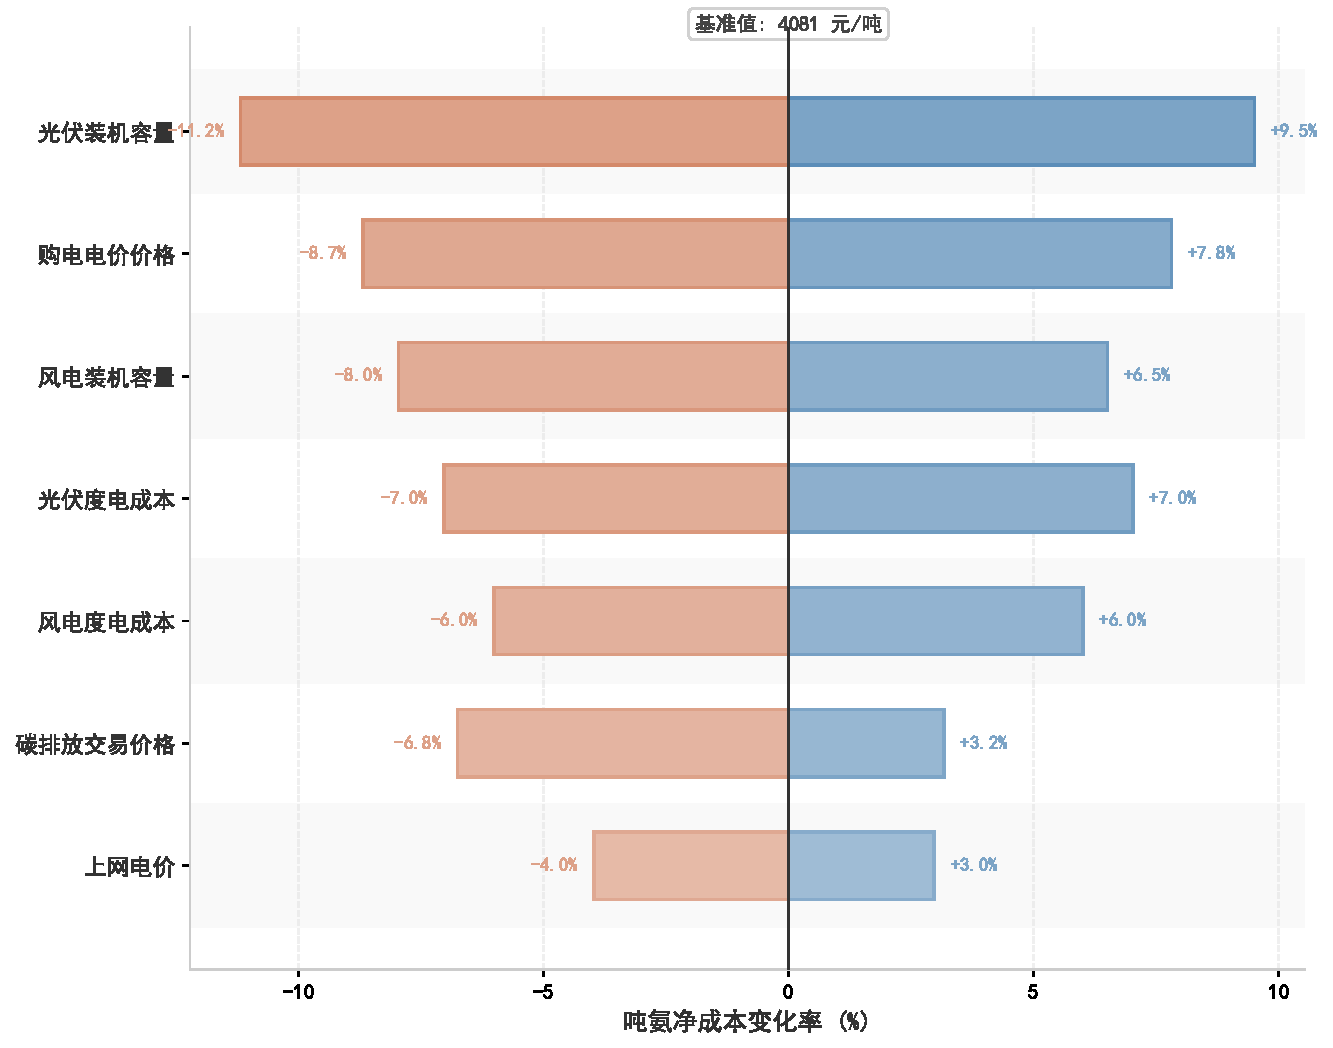
\includegraphics[width=0.9\textwidth]{figures/fig_sensitivity.pdf}
\caption{关键参数对吨氨成本的灵敏度分析}
\label{fig:sensitivity}
\end{figure}

% === DrawIO 架构图与流程图 ===
% 技术路线图
\begin{figure}[H]
\centering
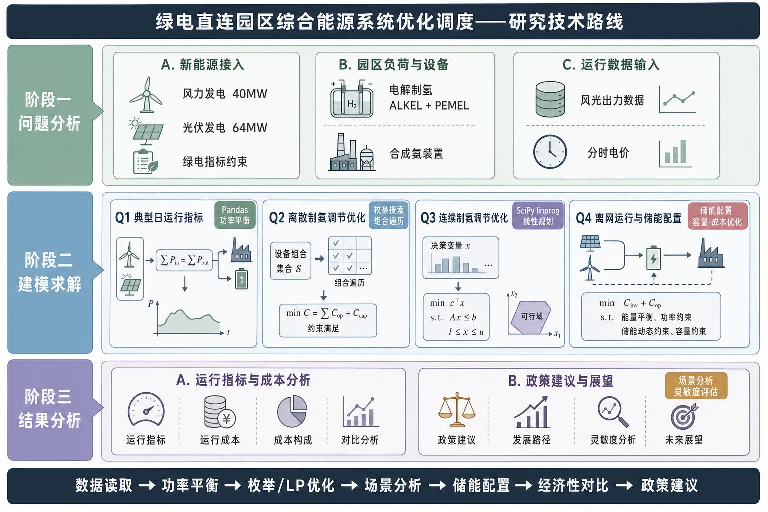
\includegraphics[width=\textwidth,height=0.45\textheight,keepaspectratio]{figures/fig_roadmap.pdf}
\caption{整体技术路线图}\label{fig:roadmap}
\end{figure}

% 园区能量流拓扑图
\begin{figure}[H]
\centering
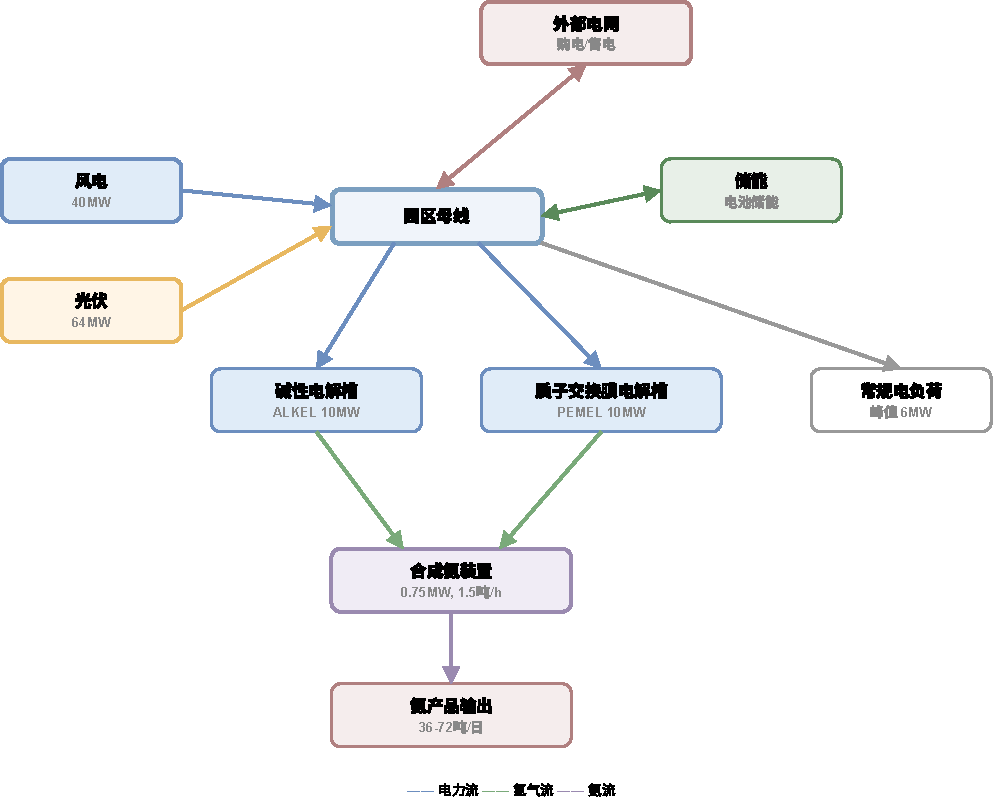
\includegraphics[width=0.9\textwidth,height=0.4\textheight,keepaspectratio]{figures/fig_energy_topology.pdf}
\caption{绿电直连型电氢氨园区能量流拓扑图}\label{fig:energy_topology}
\end{figure}

% 问题一求解流程图
\begin{figure}[H]
\centering
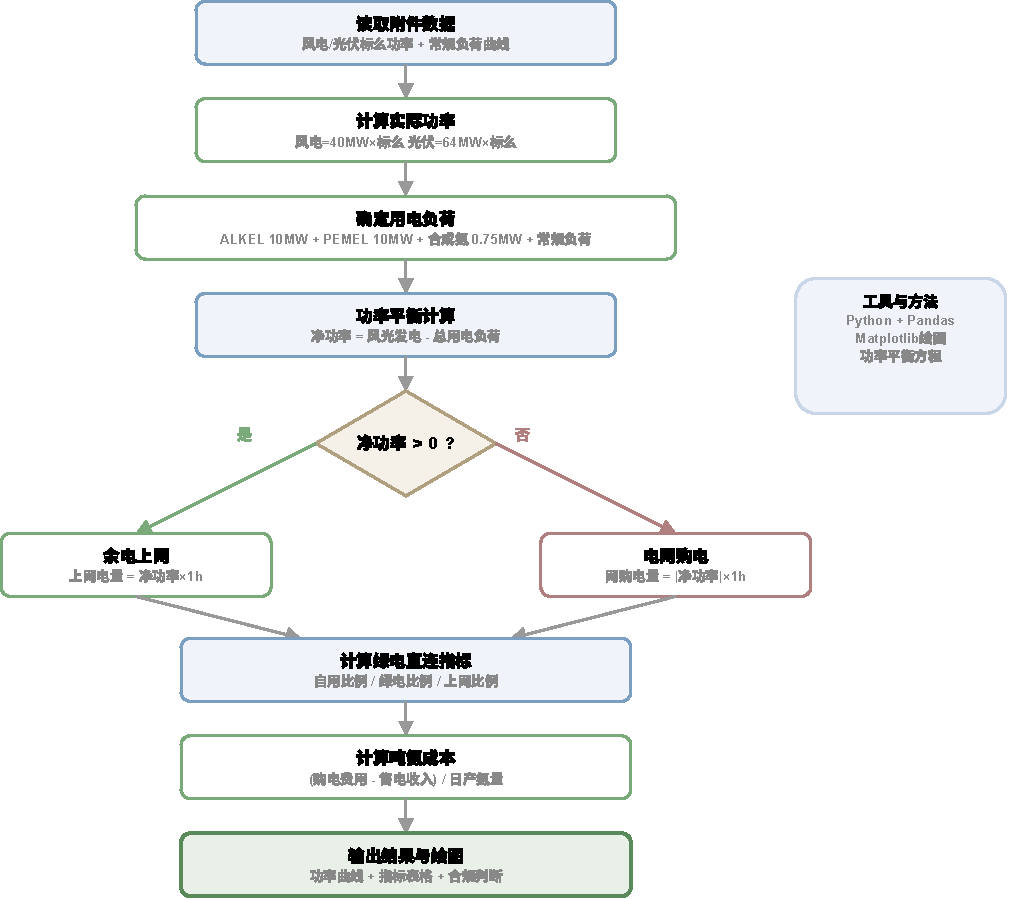
\includegraphics[width=0.85\textwidth,height=0.38\textheight,keepaspectratio]{figures/fig_flow_q1.pdf}
\caption{问题一求解流程图}\label{fig:flow_q1}
\end{figure}

% 问题二求解流程图
\begin{figure}[H]
\centering

\includegraphics[width=0.85\textwidth,height=0.38\textheight,keepaspectratio]{figures/fig_flow_q2.pdf}
\caption{问题二求解流程图}\label{fig:flow_q2}
\end{figure}

% 问题三求解流程图
\begin{figure}[H]
\centering
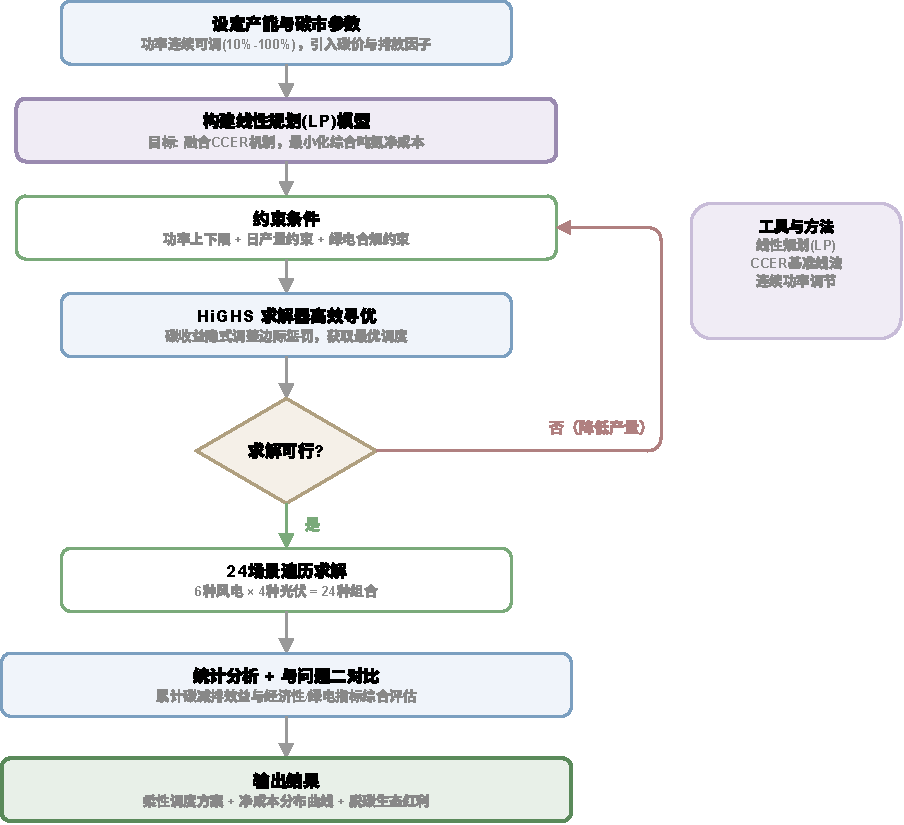
\includegraphics[width=0.85\textwidth,height=0.38\textheight,keepaspectratio]{figures/fig_flow_q3.pdf}
\caption{问题三求解流程图}\label{fig:flow_q3}
\end{figure}

% 问题四求解流程图
\begin{figure}[H]
\centering
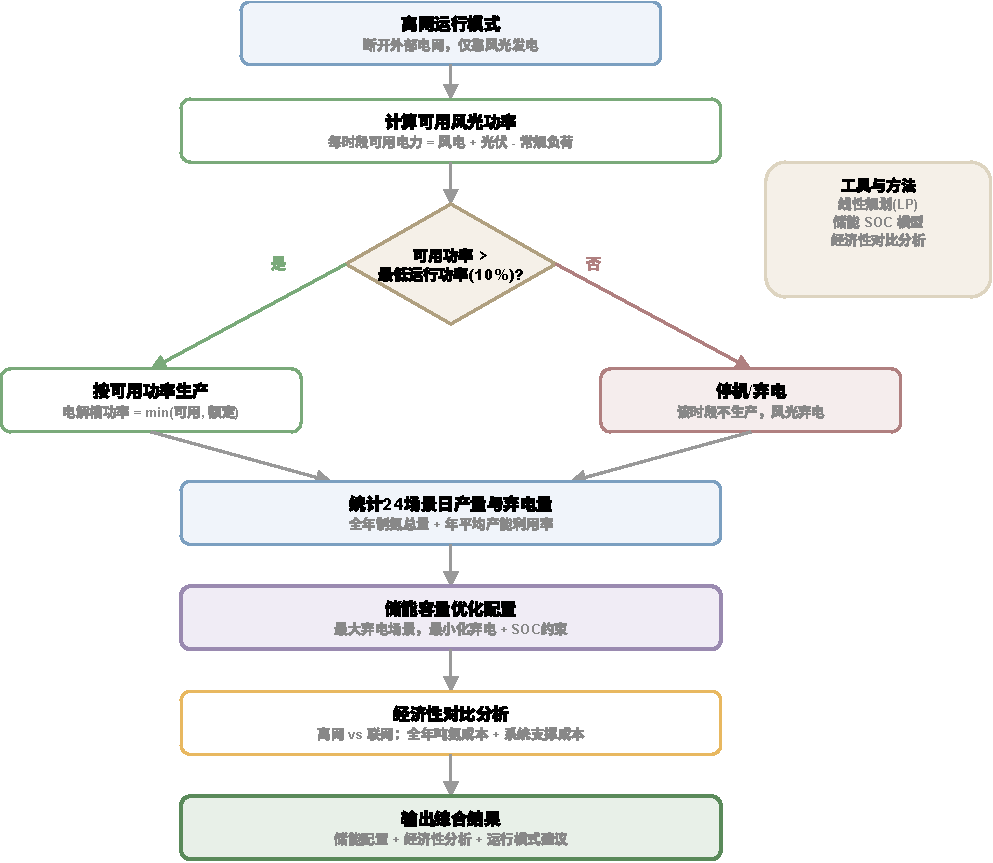
\includegraphics[width=0.85\textwidth,height=0.38\textheight,keepaspectratio]{figures/fig_flow_q4.pdf}
\caption{问题四求解流程图}\label{fig:flow_q4}
\end{figure}
